%!TEX root = ../dynamics.tex
\section{The Evolution of Amazon MTurk: 2009 to 2014}\label{sec:stats}

\subsection{Crowdsourcing Platform Dataset}\label{sec:tracker}
Over the past five years, we have periodically collected data about HITs being published on \amt\ .
Real-time data collected from the crowdsourcing platform is available at \url{http://mturk-tracker.com/}.
Interactive visualizations of the historical data are available at \url{http://xi-lab.github.io/mturk-mrkt/}.

\gd{add basic data stats, like number of hits, requesters, etc}

\subsection{A Data-driven Analysis of Platform Evolution}
\paragraph{Popular Topics  Over Time}
First we want to understand how different topics have been addressed by means of micro-task crowdsourcing over time.
In order to do such analysis we look at the tags associated with published HITs. We observe the evolution of tag popularity and associated reward on \amt\ . 
%plot explanation
Figure \ref{fig:tagEvolution} shows such behavior. Each point in the plot represent a tag associated to HITs with its frequency (i.e., number of HITs with such tag) on the x asis, its average reward of HITs with this tag on the y axis in a certain year. The path connecting data points indicates the time evolution, starting in 2009, with one point representing the tag usage over one year.
% observations
We can observe that `audio' and `transcription' tags (i.e., blue and red path from left to right) have substantially increased in frequency over time being among the most popular tags in the last two years and are paid more than \$1 on average.
HITs with the `video' tag has also increased in number with a reward that has reached a peak in 2012 and decreased after that.
HITs tagged as `categorization' have been paid constantly in the range \$0.10-\$0.30 on average, except in 2009 where they were rewarded less than \$0.1.
HITs tagged as `tweet' have not increased in number but have been paid more over years reaching \$0.9 in 2014: This can be explained by more complex tasks being requested to workers: for example, from sentiment classification to writing a tweet.

\begin{figure}[htbp]
	\centering
		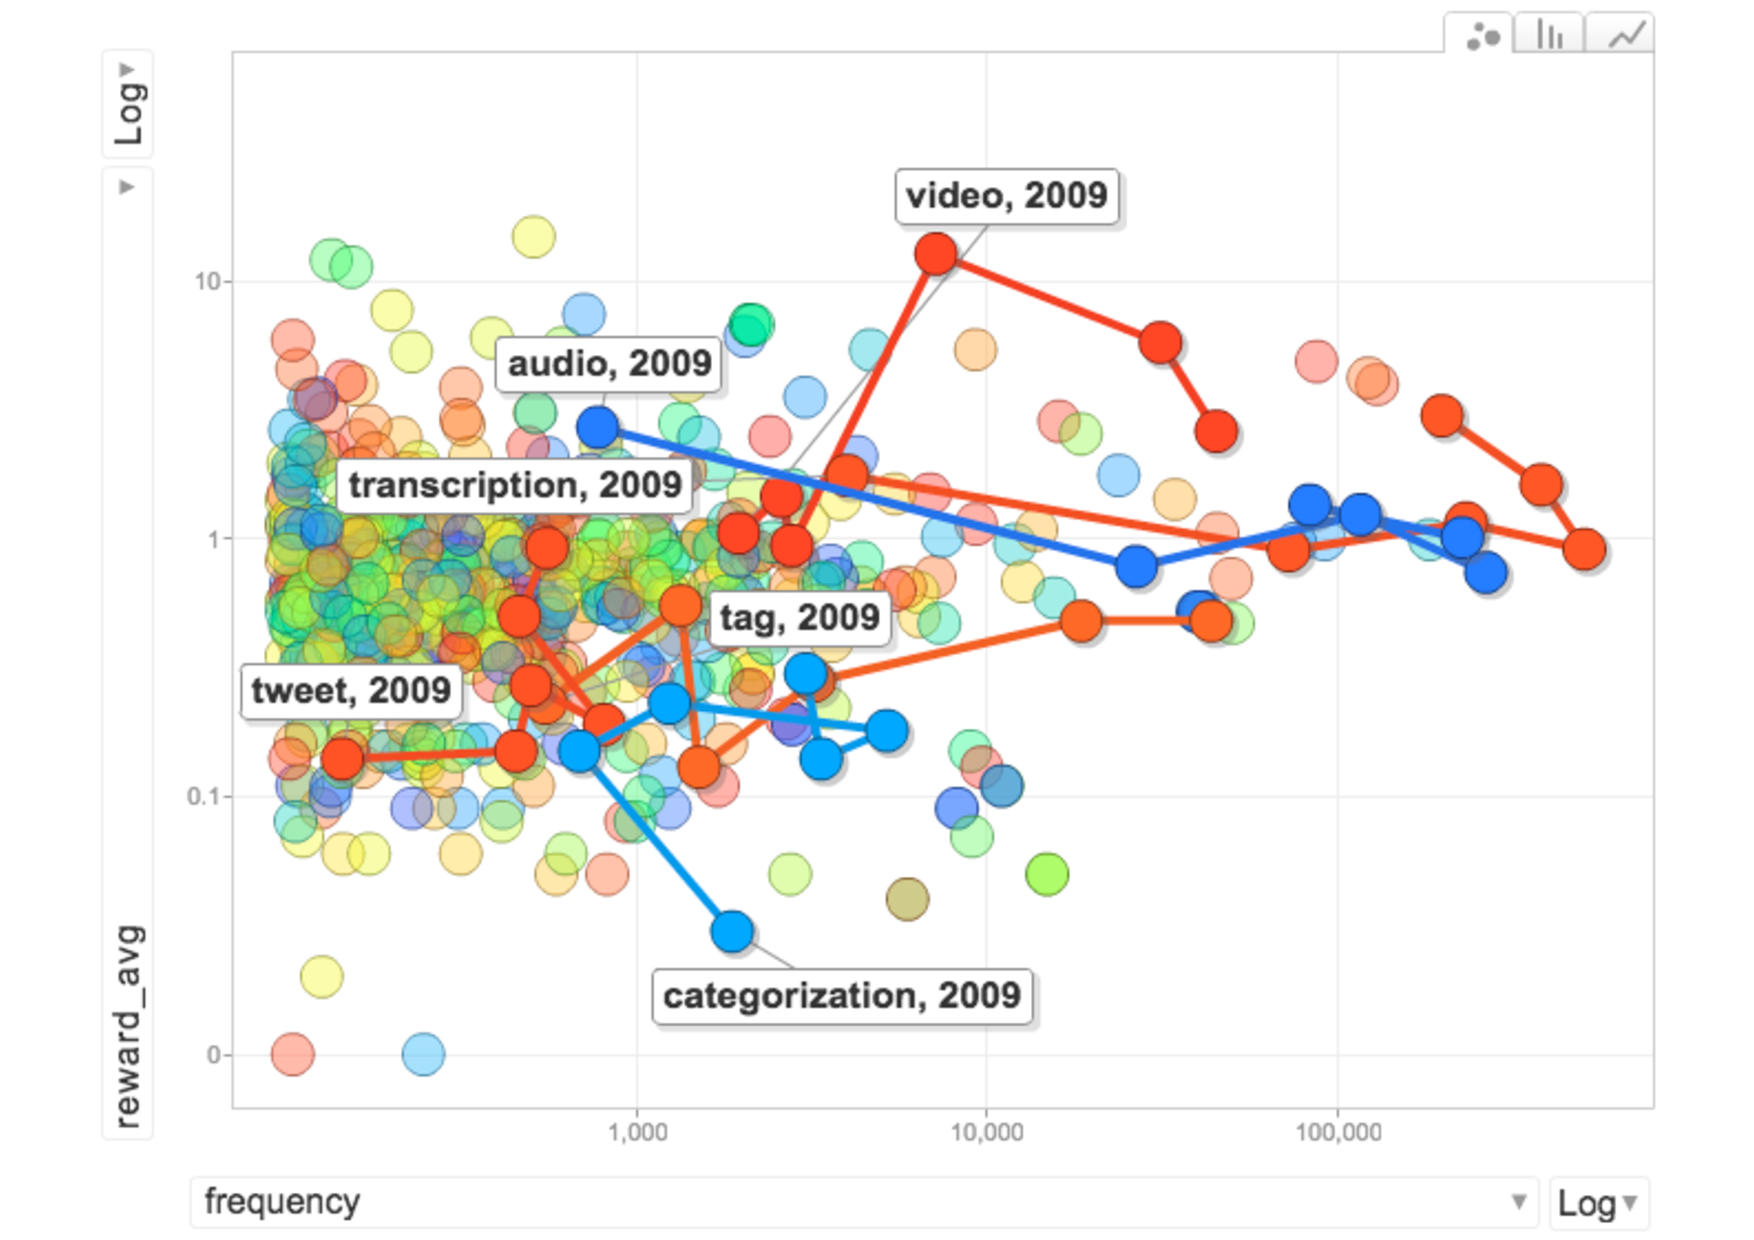
\includegraphics[width=0.5\textwidth]{figures/tagEvolution}
	\caption{tagEvolution}
	\label{fig:tagEvolution}
\end{figure}

\paragraph{Country Preference by Requesters Over Time}
Figure \ref{fig:country} shows the requirements of requesters with respect to which countries they need workers from. The left part of Figure \ref{fig:country} shows that most HITs are to be completed exclusively by workers located in US, India, or Canada. The right part of Figure \ref{fig:country} shows the evolution over time of the country requirement phenomena.
The plot shows the number of HITs with a certain country requirement (on the y axis) and its time evolution (on the x axis) with yearly steps. The size of the data point indicates the total reward associated to those HITs.
We can see that US-only HITs dominate both in terms of number as well as of reward associated to them. 
Interestingly, we notice how over time HITs uniquely for workers based in India have been decreasing. 
While HITs for workers based in Canada have been increasing over time being in 2014 more than those for workers based in India, we see that the reward associated to them is less as compared to the budget for Indian-only HITs.
As of 2014, both HITs for workers based in Canada or UK are more numerous that those for workers based in India.

\gd{how many HITs have country filters and how many have no country filter in percentage?} 

\begin{figure*}[htbp]
	\centering
		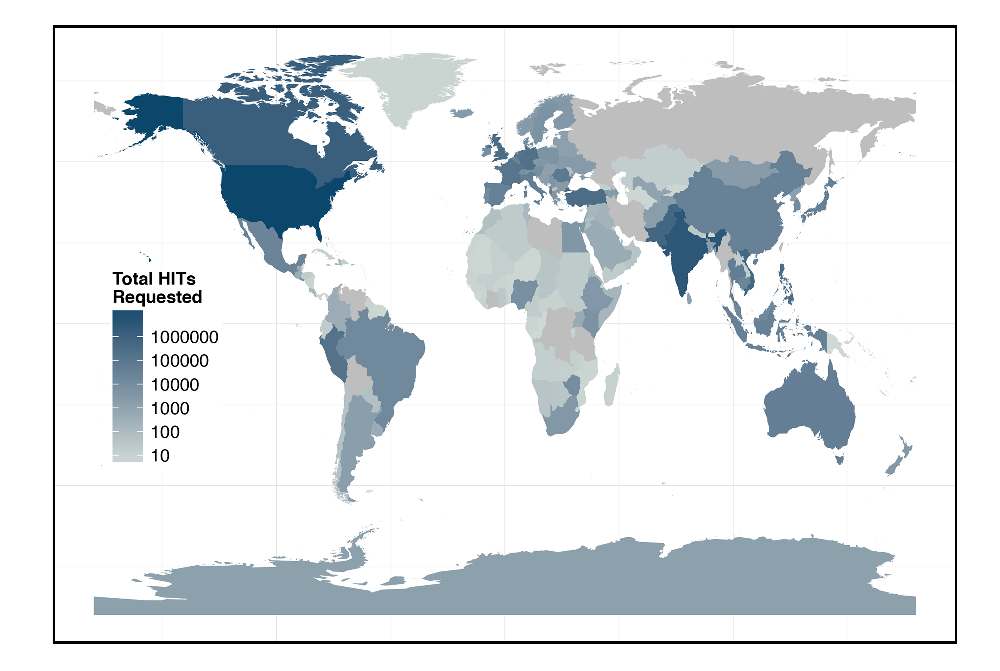
\includegraphics[width=0.48\textwidth]{figures/map}
		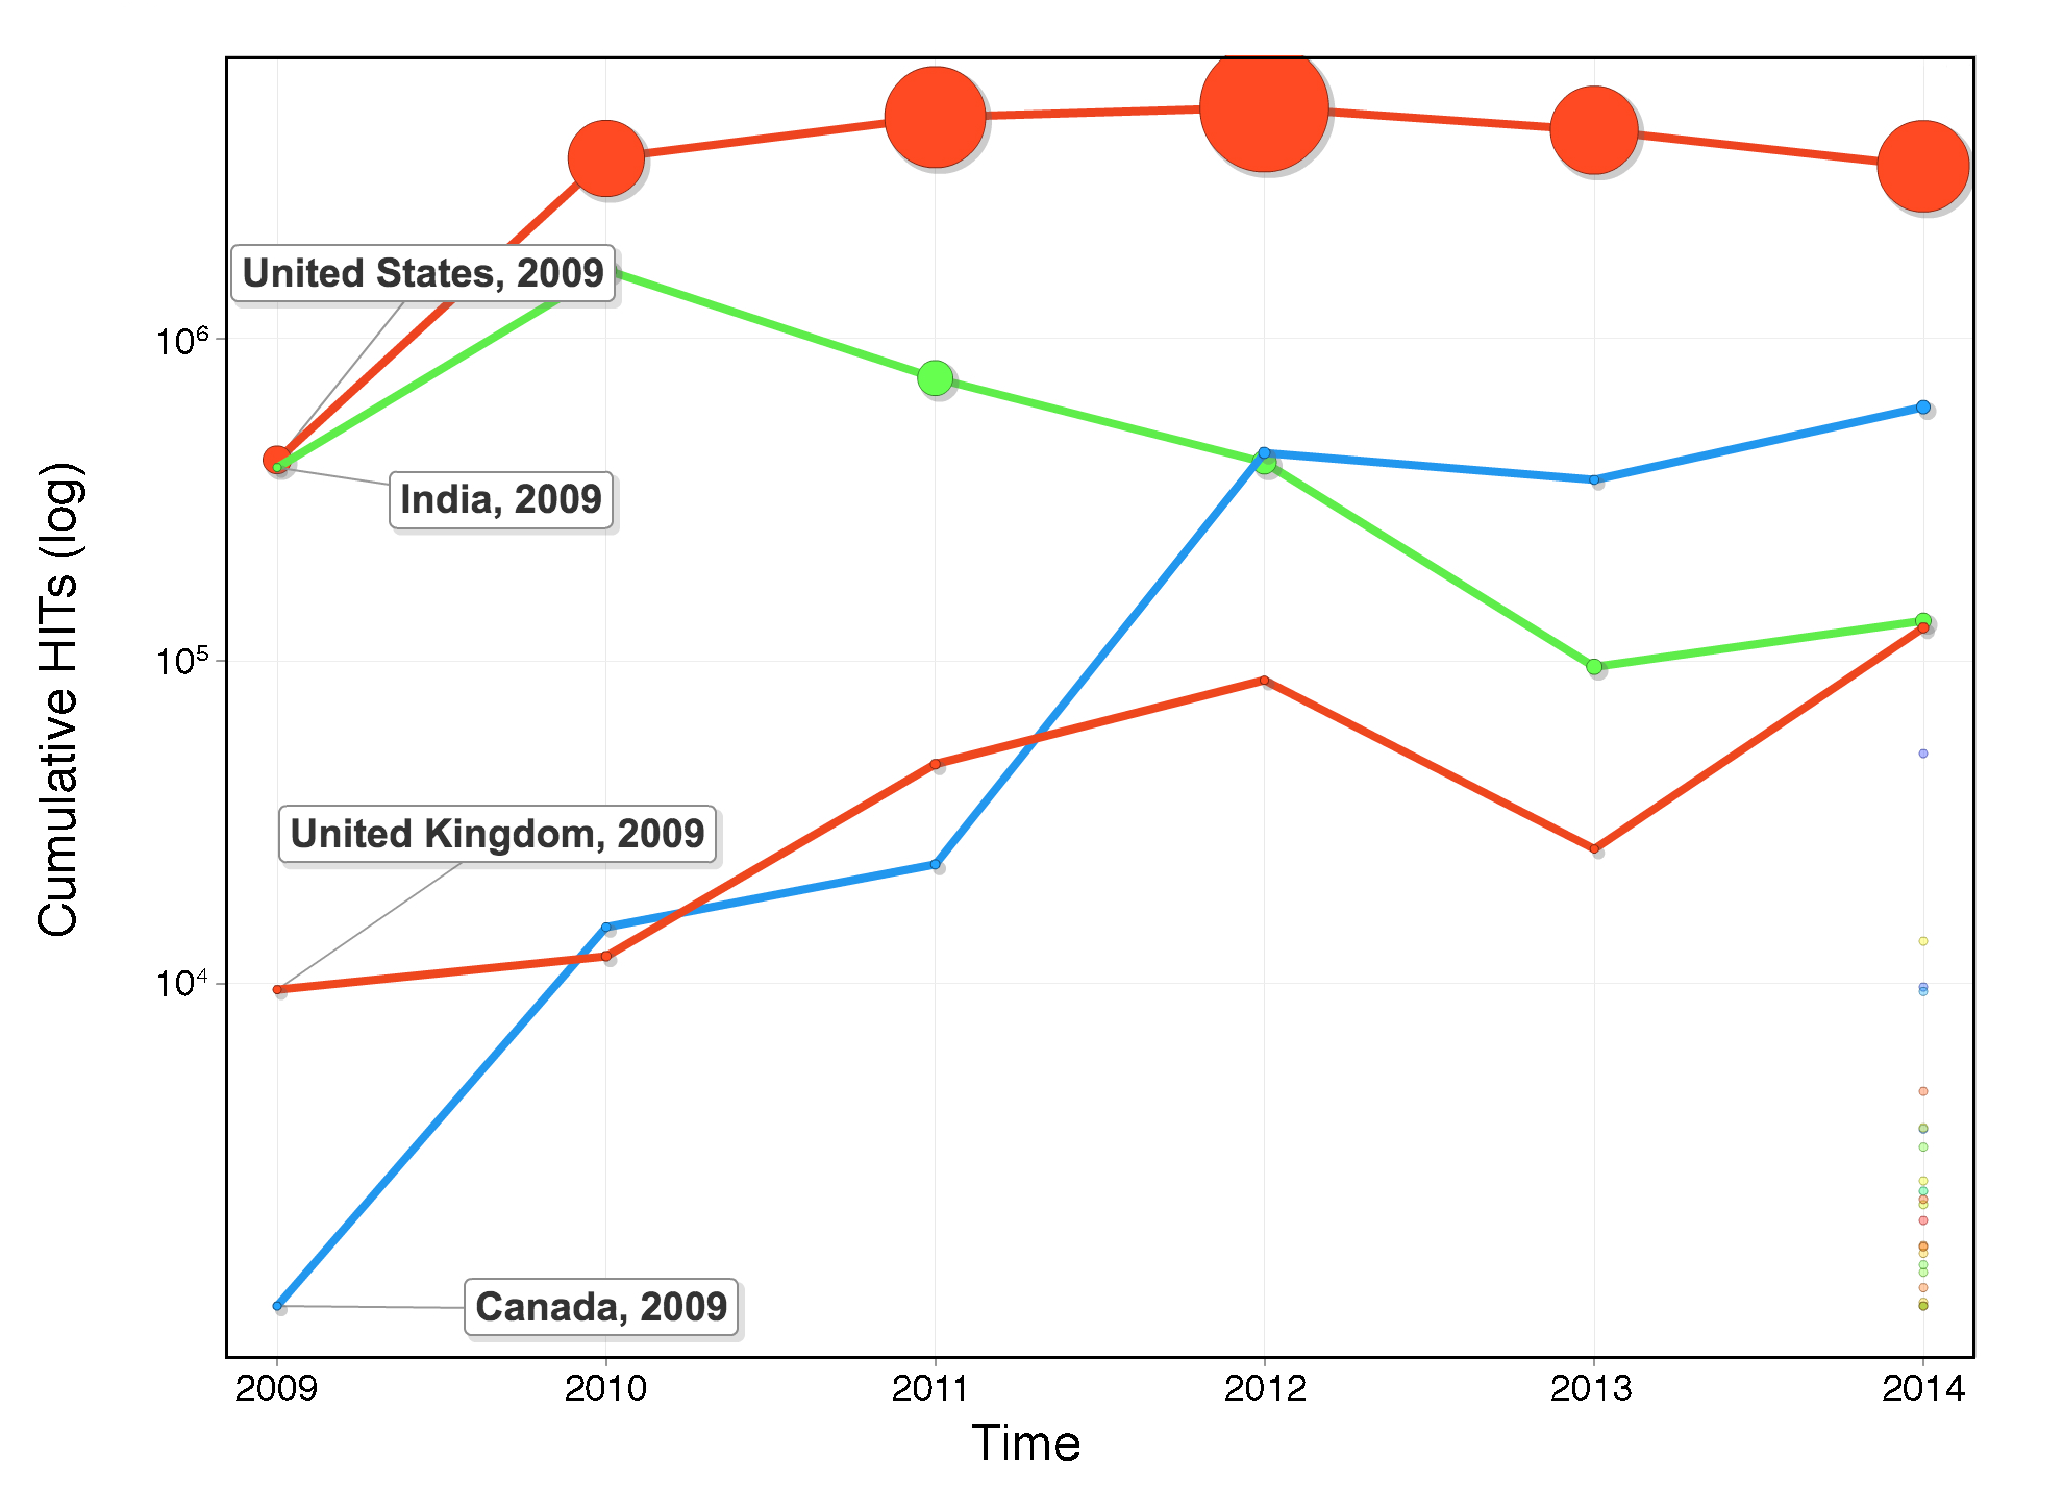
\includegraphics[width=0.48\textwidth]{figures/countriesTime}
	\caption{HITs with specific country requirements. On the left, the countries with most HITs dedicated to them. On the right, the time evolution (x-axis) of country specific HITs with volume (y-axis) and reward information (size of data point).}
	\label{fig:country}
\end{figure*}


% \subsection{Why Did Certain Requesters Quit?}
% \subsection{Does reputation Improve Throughput?}

\paragraph{HIT Reward Analysis}
\begin{figure}[htbp]
	\centering
		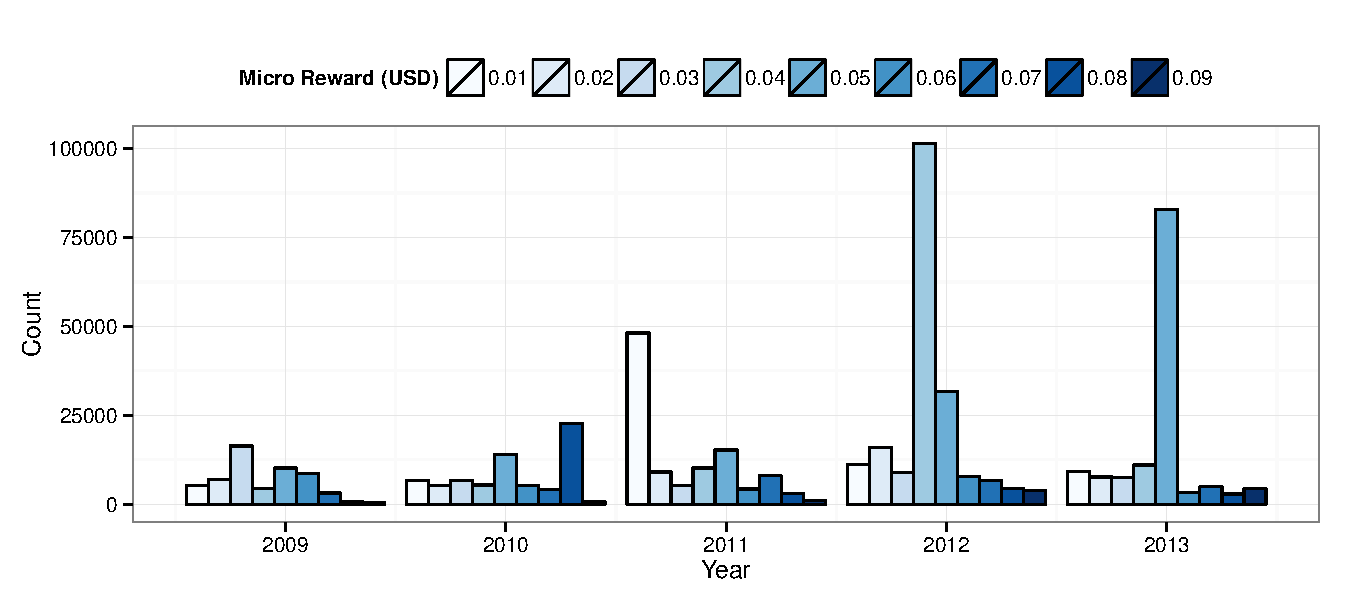
\includegraphics[width=0.5\textwidth]{figures/reward_year}
	\caption{Reward \gd{can we add 2014?}}
	\label{fig:reward_year}
\end{figure}

\begin{figure}[htbp]
	\centering
		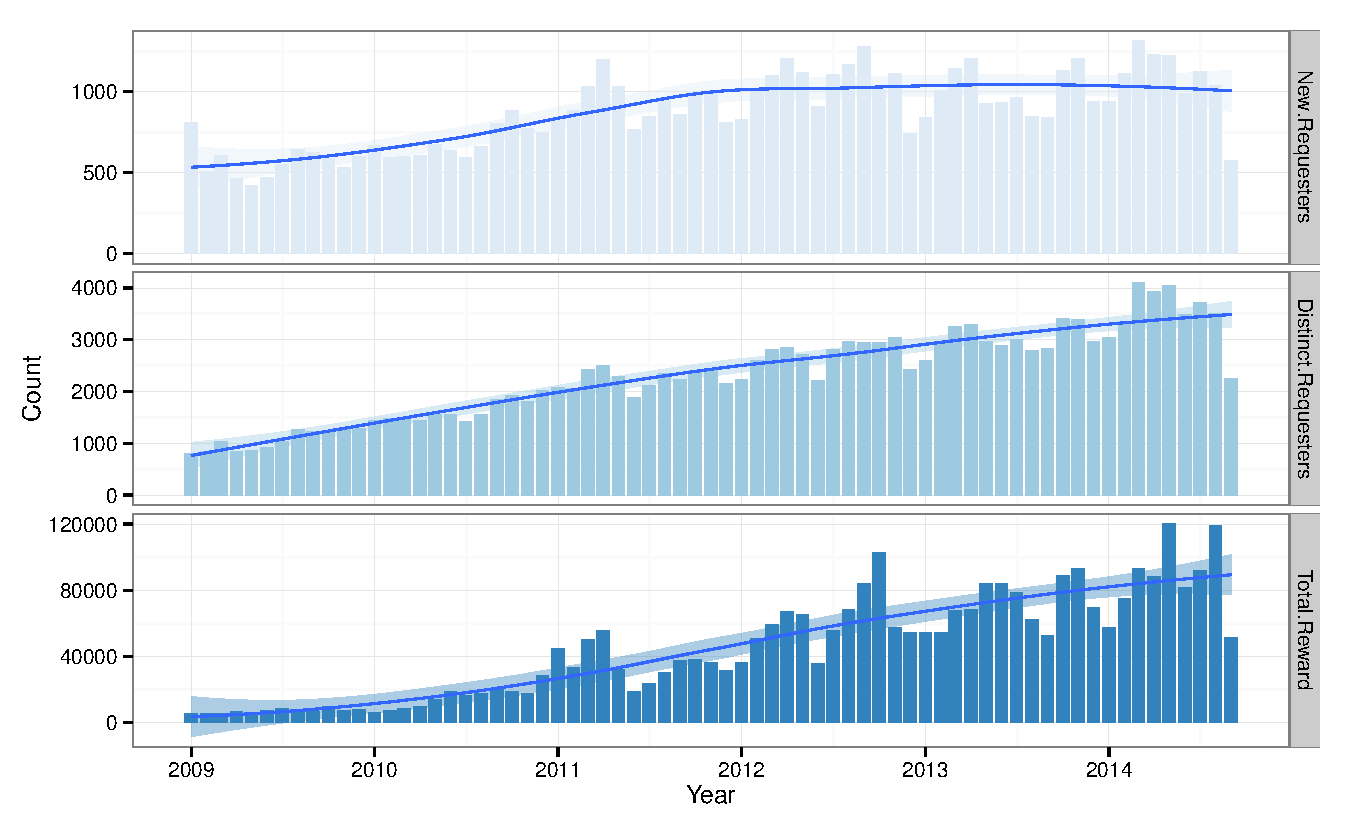
\includegraphics[width=0.5\textwidth]{figures/requesters_reward}
	\caption{Reward and Requesters}
	\label{fig:requesters_reward}
\end{figure}



\begin{figure}[htbp]
	\centering
		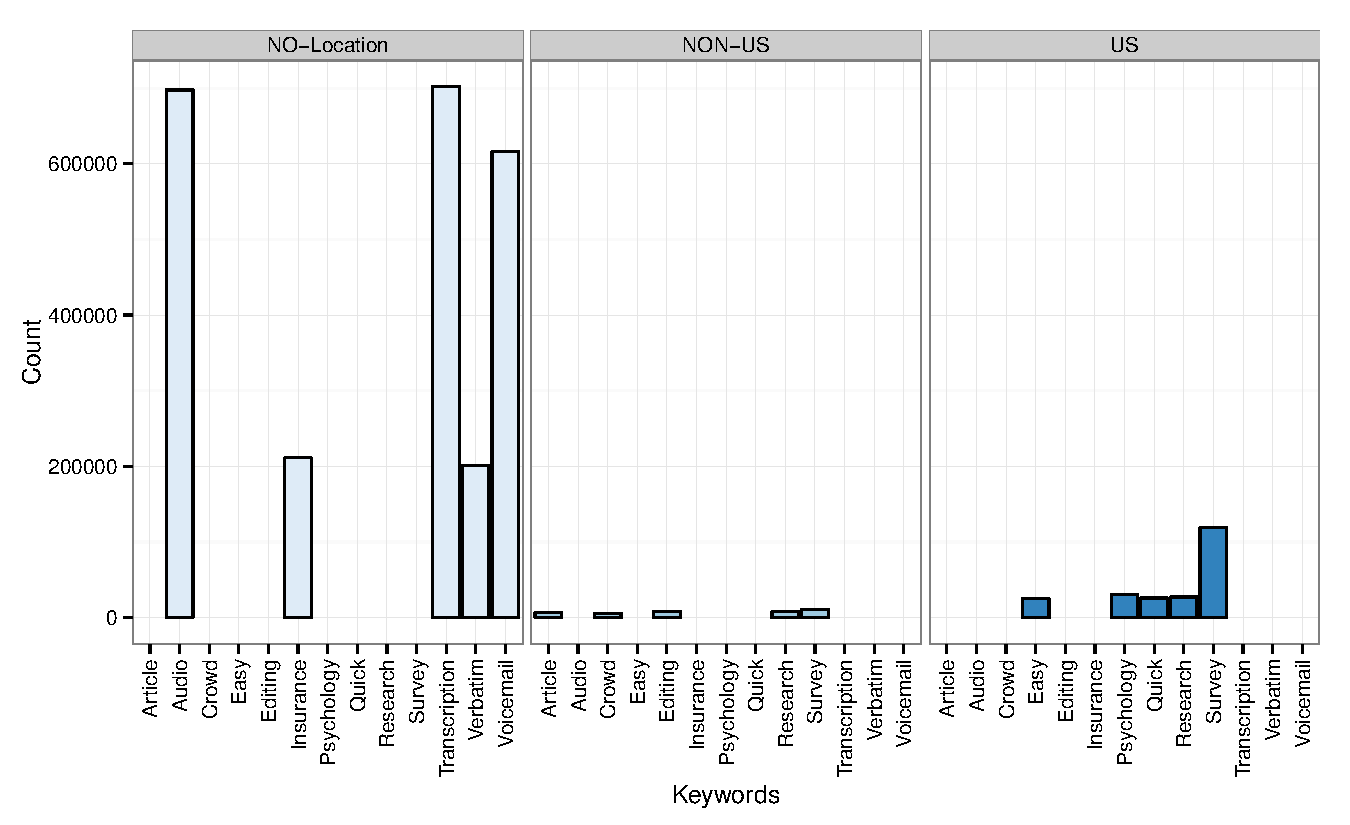
\includegraphics[width=0.5\textwidth]{figures/keywords_location}
	\caption{Keywords vs Location}
	\label{fig:keyword_loc}
\end{figure}

\begin{figure}[htbp]
	\centering
		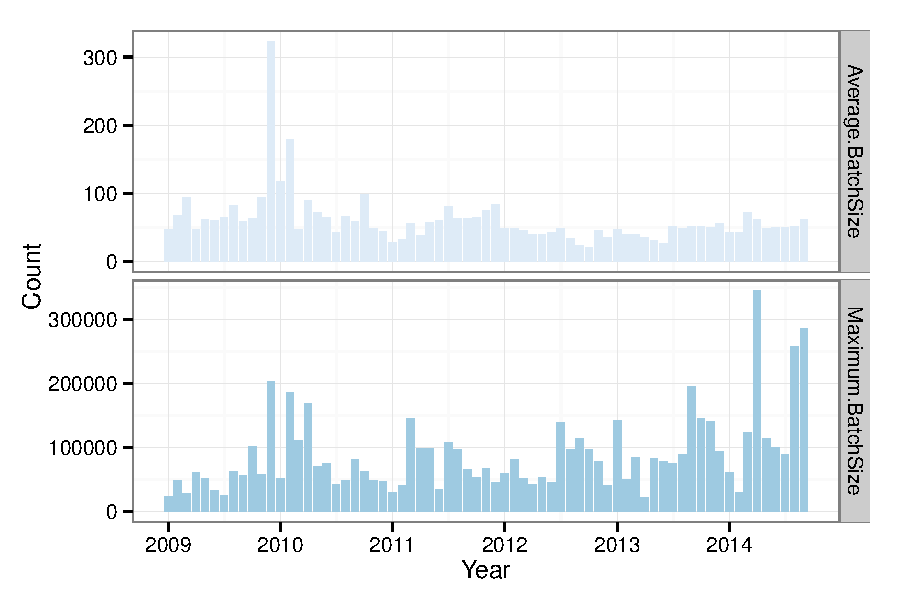
\includegraphics[width=0.5\textwidth]{figures/batch_size}
	\caption{Batch Sizes}
	\label{fig:batch_size}
\end{figure}


